\documentclass[12pt, aspectratio=43]{beamer}
\setbeamerfont{frametitle}{size=\normalsize}

\usetheme[secheader]{Hannover}
\usecolortheme{dolphin}
\usepackage[T1]{fontenc}                       % allow Latin1 characters
\usepackage[latin1]{inputenc}
\setbeamerfont{title in sidebar}{size=\fontsize{8}{7}\selectfont}
\setbeamerfont{section in sidebar}{size=\fontsize{8}{10}\selectfont}
\usepackage{lmodern}
\usepackage[natbib,citestyle=authoryear]{biblatex}
\setbeamertemplate{navigation symbols}{}
\usepackage{multicol}
\usepackage{listings}
\usepackage{multimedia}
\usepackage{xcolor}


\addbibresource{scivis.bib}

\renewcommand{\footnote}{\arabic{footnote}}
\newcommand{\slide}[2]{\frame{
	\frametitle{#1}#2
}}

\lstset{basicstyle=\scriptsize, language=python,
                keywordstyle=\color{blue}\ttfamily,
                stringstyle=\color{red}\ttfamily,
                commentstyle=\color{magenta}\ttfamily,
                morecomment=[l][\color{magenta}]{\#}}



\DefineBibliographyStrings{english}{%
  references = {Refs.},% replace "references" with Refs.
}

\title{Scientific visualization (with Python)}

%\input{atalhos.tex}

\author[]{Tom�s Chor}
\date{\today} 
\institute[]{}

\setbeamertemplate{footline}{\hfill\insertframenumber / \inserttotalframenumber}

\begin{document}
\slide{}{\titlepage}

\section{Basics}

\slide{Introduction}{
\begin{multicols}{2}
\begin{itemize}
\item Many plotting systems to choose from
\begin{itemize}
\item matplotlib
\item gnuplot
\item paraview
\item scilab
\item basemap
\item matlab
\item techplot
\end{itemize}
\vfill\null
\columnbreak
\item They can serve many purposes
\begin{itemize}
\item quick glance at data
\item presentation to others
\item scientific publication
\item general public
\end{itemize}
\end{itemize}
\end{multicols}}

\slide{Introduction}{
\begin{itemize}
\item The nature of the plot depends on the nature of data
\begin{itemize}
\item gridded data
\item sparse data
\item dimensionality ($f(x)$, $f(x,y)$, $f(x,y,t)$ ...)
\end{itemize}
\item Interactive plots are becoming very easy to make, but we won't focus on it
\item Checkout basemap (python) for map-projection plotting
\end{itemize}

}

\slide{We have to get subjective}{
Some general subjective rules to aim for
\begin{itemize}
\item clarity
\item precision
\item efficiency
\end{itemize}
}

\slide{It might be subjective, but we can tell the difference}{
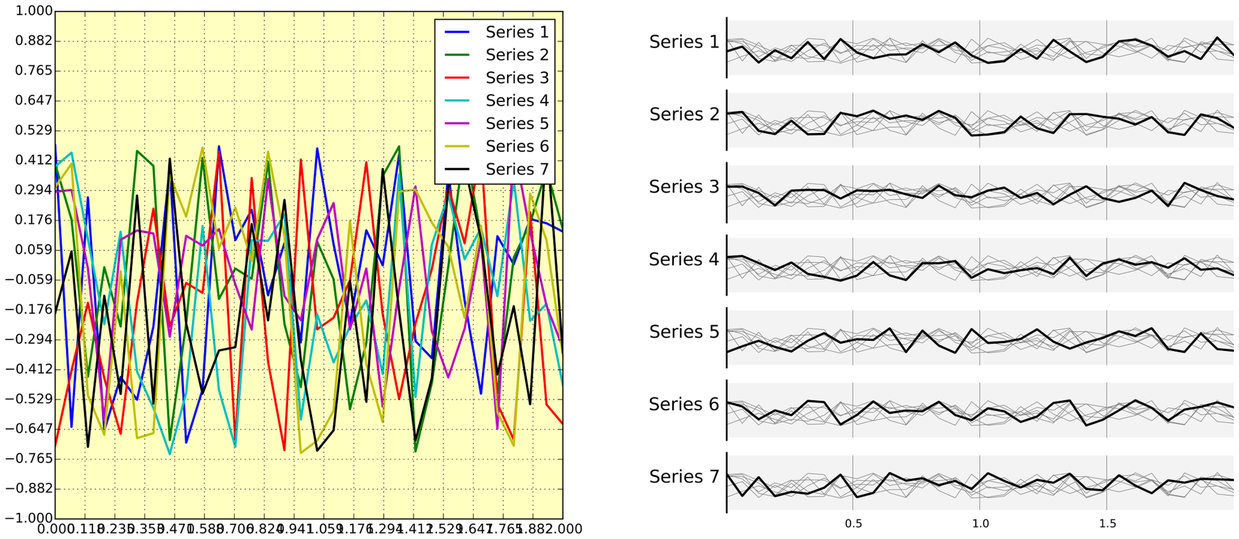
\includegraphics[width=\textwidth]{plots/chartjunk2.png}
\vspace{1cm}
Reproduced from \citet{rougier.ea2014}. (Although notice that there should be
labels in the plot!)
}

\slide{}{
If you're showing more than one plot on that are meant to be compared, keep the same scales
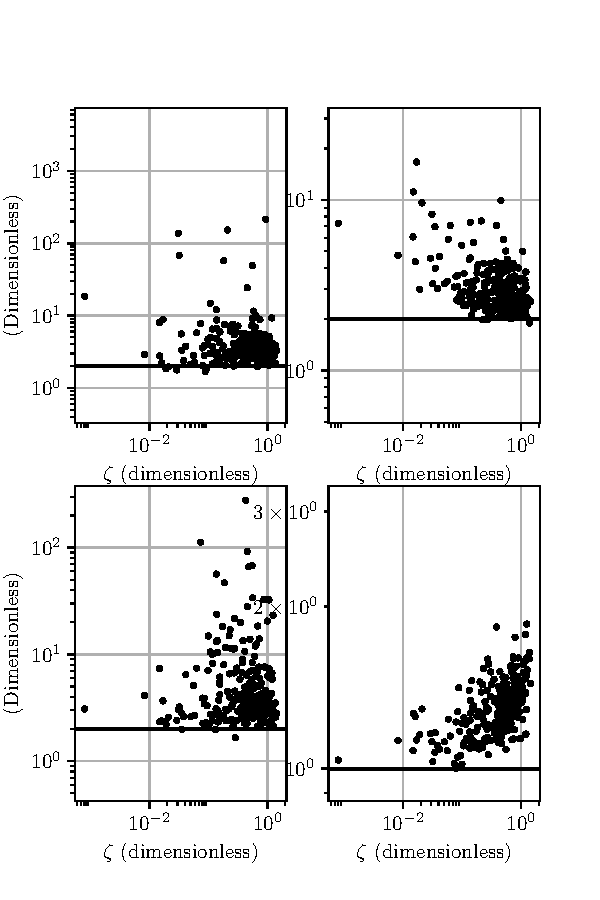
\includegraphics[width=.5\textwidth]{plots/subplots/bad_subplots.pdf}
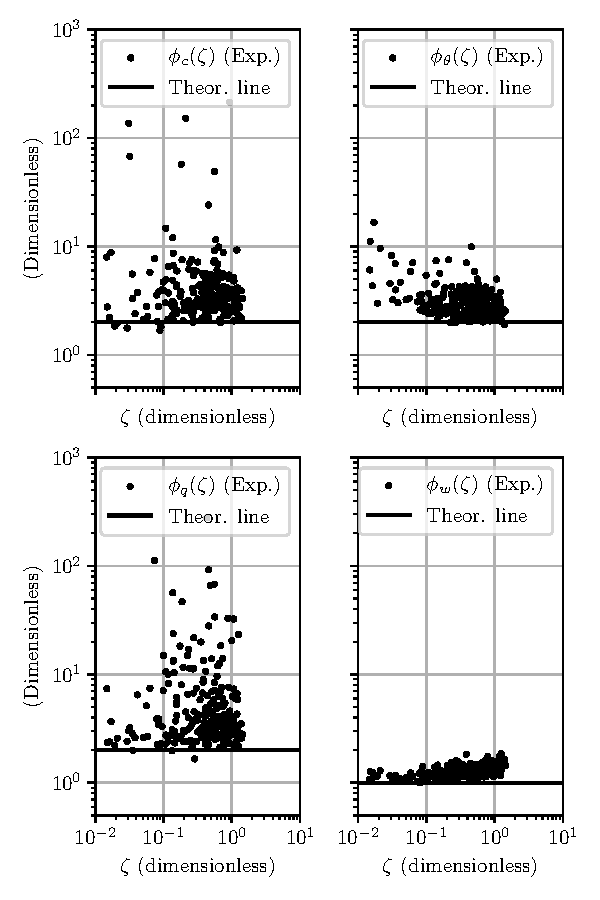
\includegraphics[width=.5\textwidth]{plots/subplots/good_subplots.pdf}
}


\slide{Make your message easy with your plot}
{
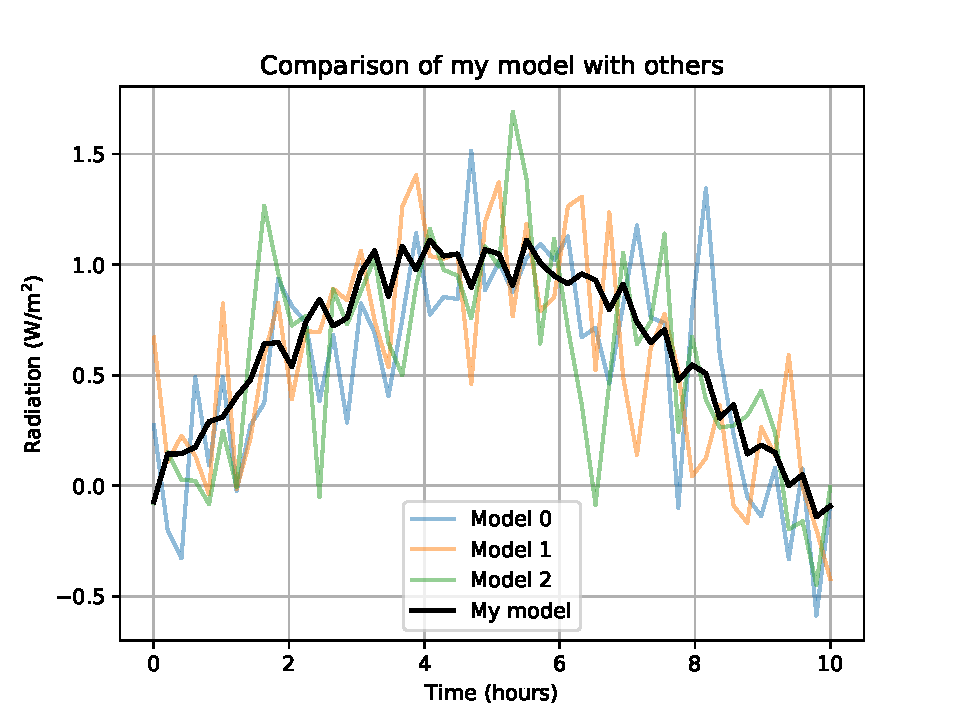
\includegraphics[width=.9\textwidth]{plots/ex1/ex1.pdf}}



\section{1D data}

\slide{}{
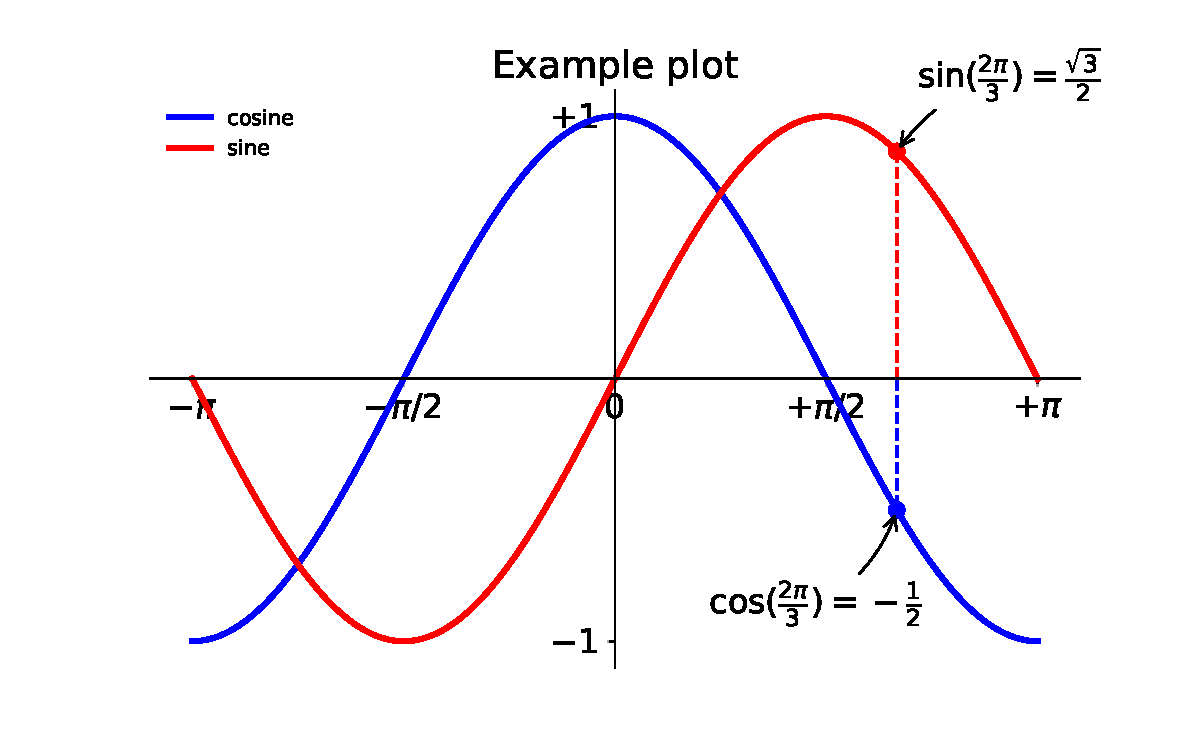
\includegraphics[width=.99\textwidth]{plots/1D_ex0/1D_ex.pdf}

Taken from \citet{rougier2015}.
\begin{multicols}{2}
\begin{itemize}
\item Curves
\item Labels
\item Ticks (and labels)
\item Title
\item Legend
\item Other helpful marks
\end{itemize}
\end{multicols}
}

\slide{Some things are almost mandatory}{
Every plot should be self-sufficient in its content. So they should include
\begin{itemize}
\item labels
\item units (scientific world uses metric)
\item legends
\end{itemize}
}

\slide{}{
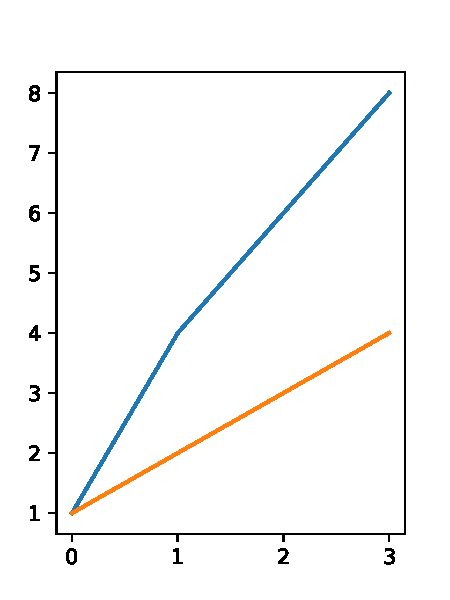
\includegraphics[width=.5\textwidth]{plots/ex0/bad_ex.pdf}
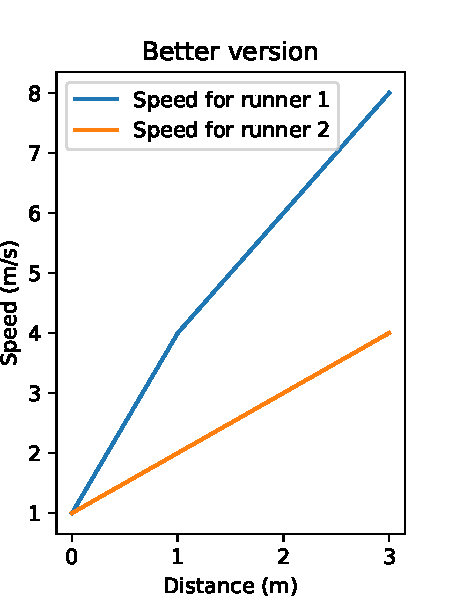
\includegraphics[width=.5\textwidth]{plots/ex0/good_ex.pdf}
}



\subsection{Semilog plot}
\slide{Log-Lin plots}{
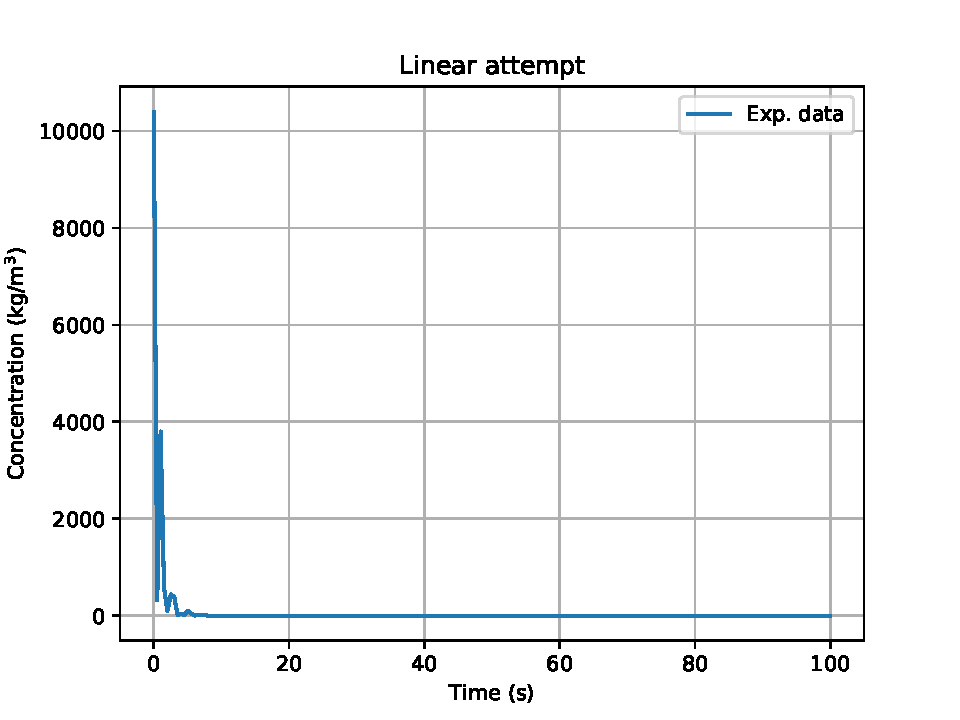
\includegraphics[width=.95\textwidth]{plots/semilogy/linlin_exp_decay.pdf}}

\begin{frame}[fragile]{Log-Lin plots}
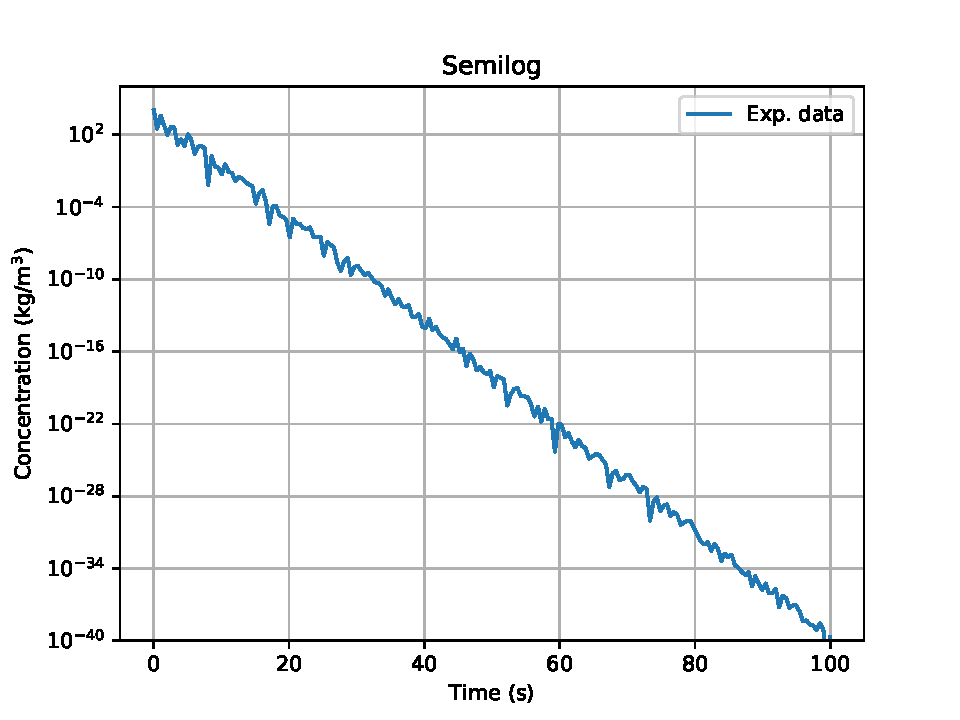
\includegraphics[width=.95\textwidth]{plots/semilogy/semiy_exp_decay.pdf}
\begin{lstlisting}[language=python]
plt.semilogy(X, Y)
\end{lstlisting}
\end{frame}


\begin{frame}[fragile]{Log-Lin plots}
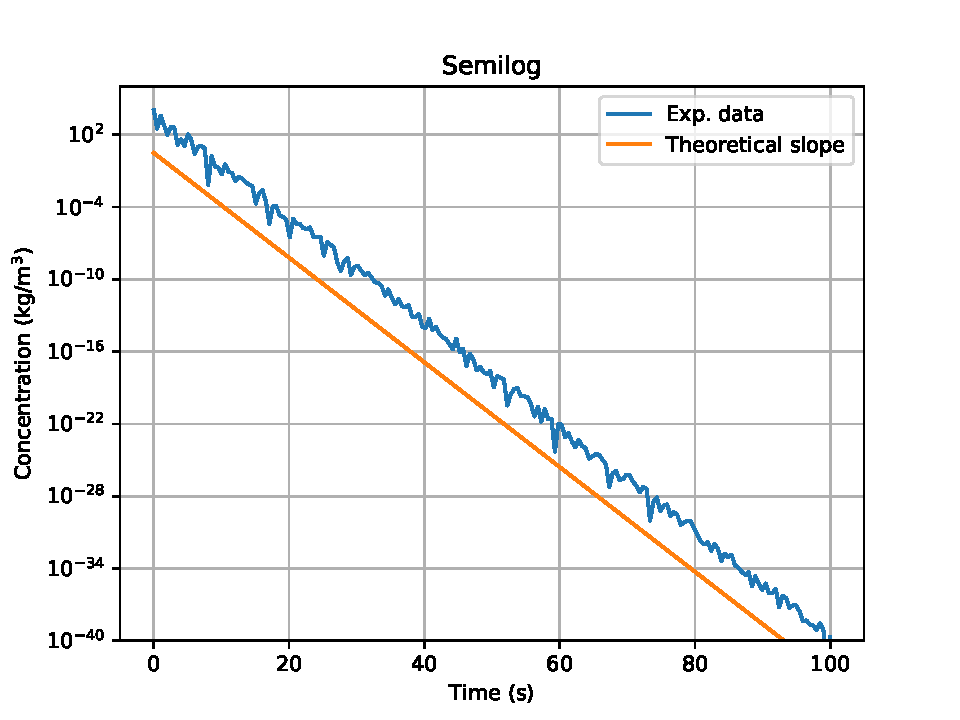
\includegraphics[width=.95\textwidth]{plots/semilogy/semiy_exp_decay2.pdf}
\begin{lstlisting}[language=python]
plt.semilogy(X, Y)
\end{lstlisting}
\end{frame}


\slide{Log-Lin plots}{
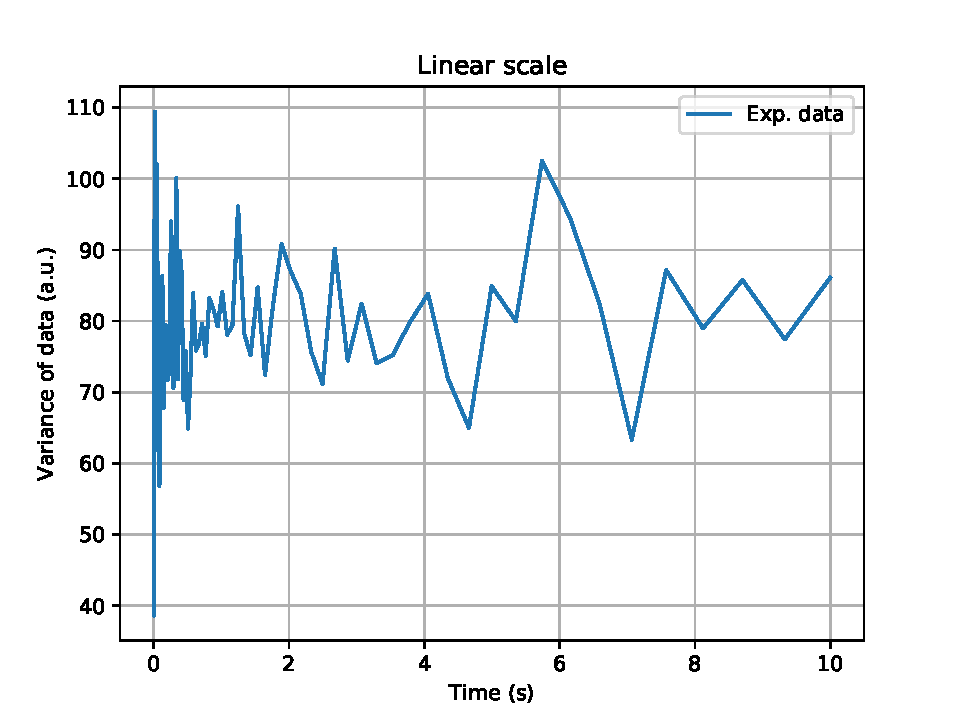
\includegraphics[width=.95\textwidth]{plots/semilogx/semix_lin.pdf}}

\begin{frame}[fragile]{Log-Lin plots}
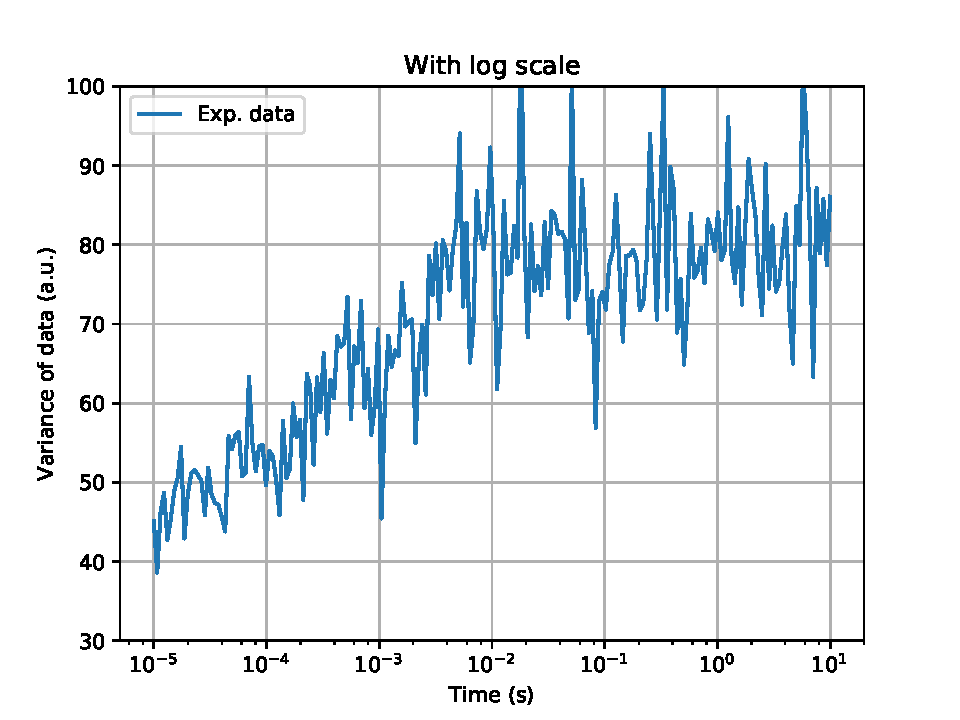
\includegraphics[width=.95\textwidth]{plots/semilogx/semix_semix.pdf}
\begin{lstlisting}[language=python]
plt.semilogx(X, Y)
\end{lstlisting}
\end{frame}

\begin{frame}[fragile]{Log-Lin plots}
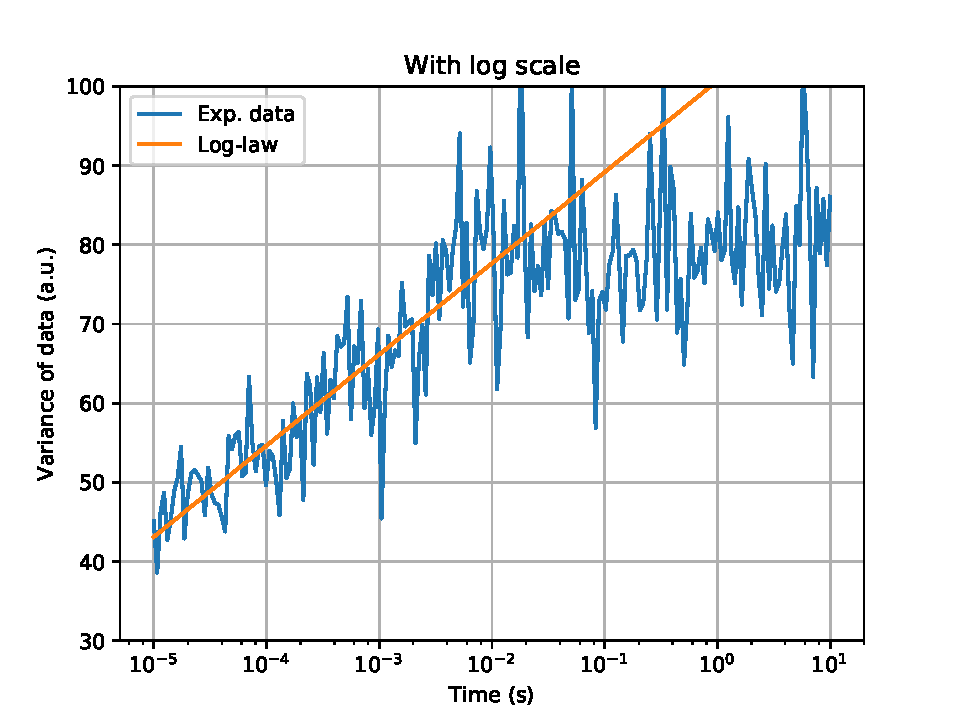
\includegraphics[width=.95\textwidth]{plots/semilogx/semix_semix2.pdf}
\begin{lstlisting}[language=python]
plt.semilogx(X, Y)
\end{lstlisting}
\end{frame}



\subsection{Log plot}
\slide{Log-Log plots}{
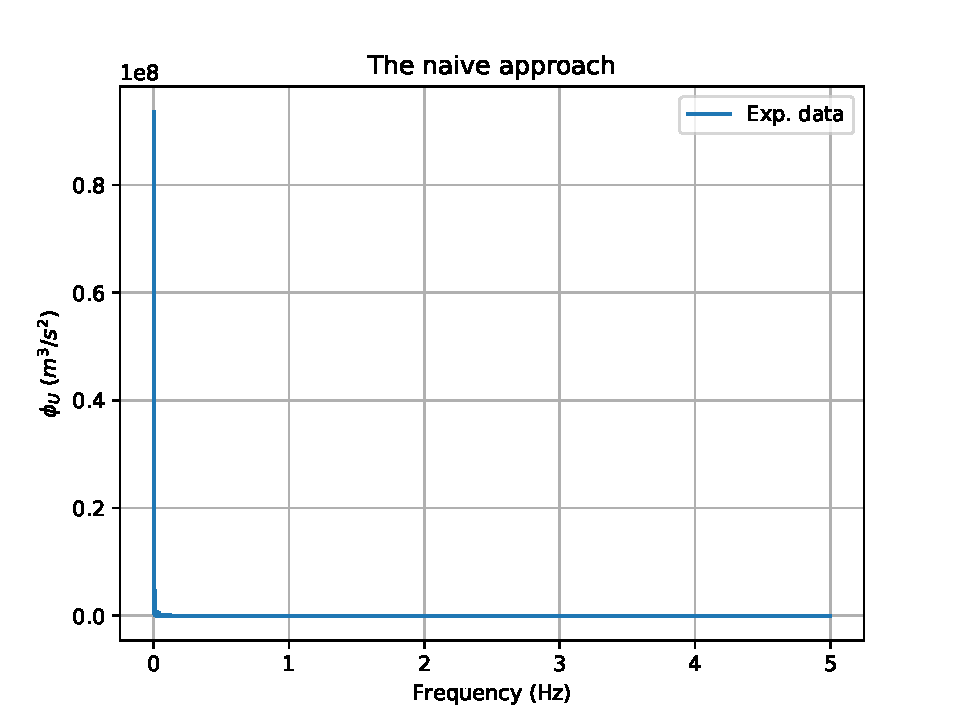
\includegraphics[width=\textwidth]{plots/loglog/linlin_Uspec.pdf}}

\begin{frame}[fragile]{Log-Log plots}
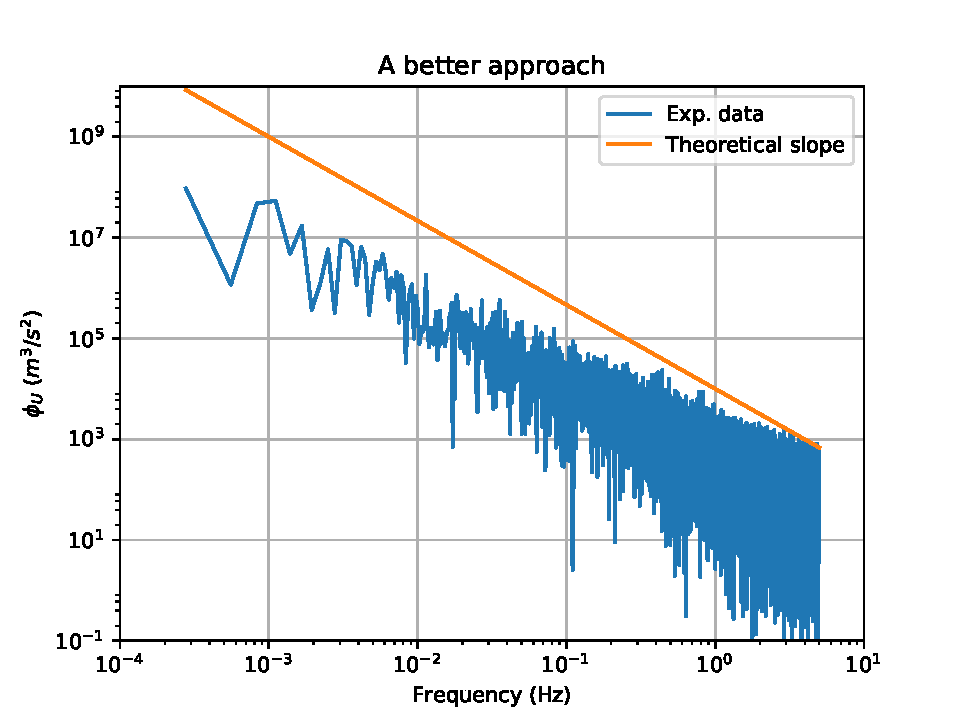
\includegraphics[width=.9\textwidth]{plots/loglog/loglog_Uspec.pdf}
\begin{lstlisting}[language=python]
plt.loglog(X, Y)
\end{lstlisting}
\end{frame}

\begin{frame}[fragile]{Binning}
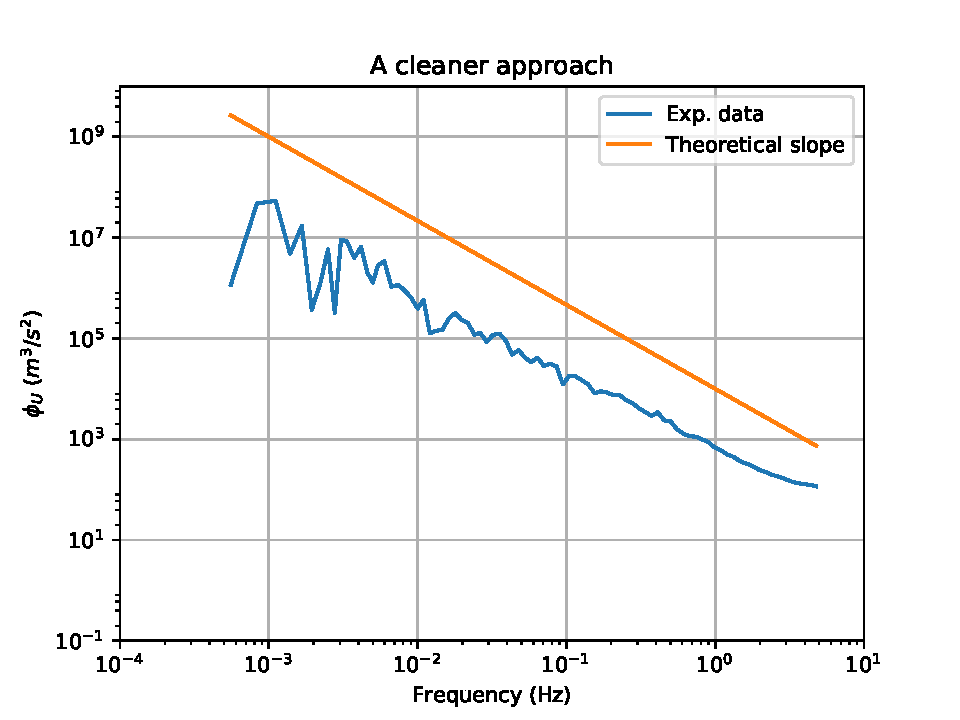
\includegraphics[width=.9\textwidth]{plots/loglog/loglog2_Uspec.pdf}
\begin{lstlisting}[language=python]
plt.loglog(X, Y)
\end{lstlisting}
\end{frame}


\begin{frame}[fragile]{Binning and errorbars}
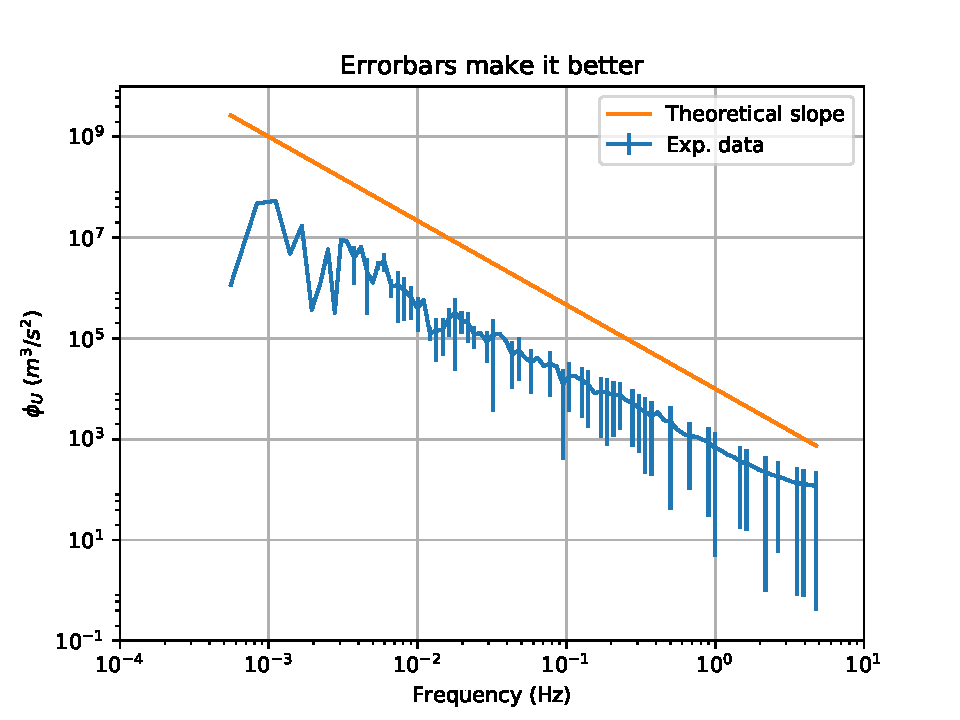
\includegraphics[width=.9\textwidth]{plots/loglog/loglog3_Uspec.pdf}
\begin{lstlisting}[language=python]
plt.errorbar(X, Y, yerr=yerrors, xerr=xerrors)
plt.yscale('log')
plt.xscale('log')
\end{lstlisting}
\end{frame}

\subsection{PDF}
\begin{frame}[fragile]{Creating a Prob. Dens. Function (and using \LaTeX)}
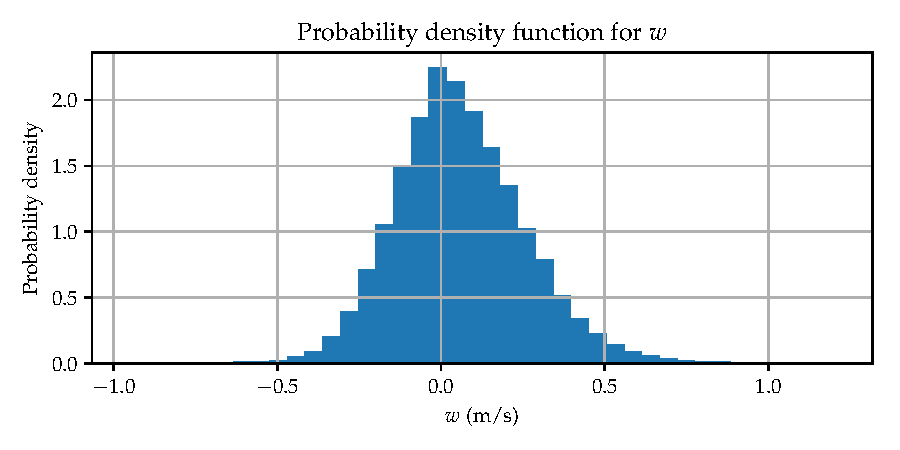
\includegraphics[width=.95\textwidth]{plots/pdf/pdf.pdf}
\begin{lstlisting}
from matplotlib import rc
rc('font', family='serif', serif='Palatino')
rc('text', usetex=True)
PDF, bin_edges = np.histogram(W, bins=40, density=True)
bin_mid = (bin_edges[:-1]+bin_edges[1:])/2
plt.bar(bin_mid,PDF, width=width)
\end{lstlisting}
\end{frame}




\section{2D data}

\slide{Plotting 2D data}{
Two more things to worry about when plotting 2D data

\begin{itemize}
\item Type of plot
\item Colorbar
\end{itemize}
}


\subsection{Types of plot (scalars)}


\begin{frame}[fragile]
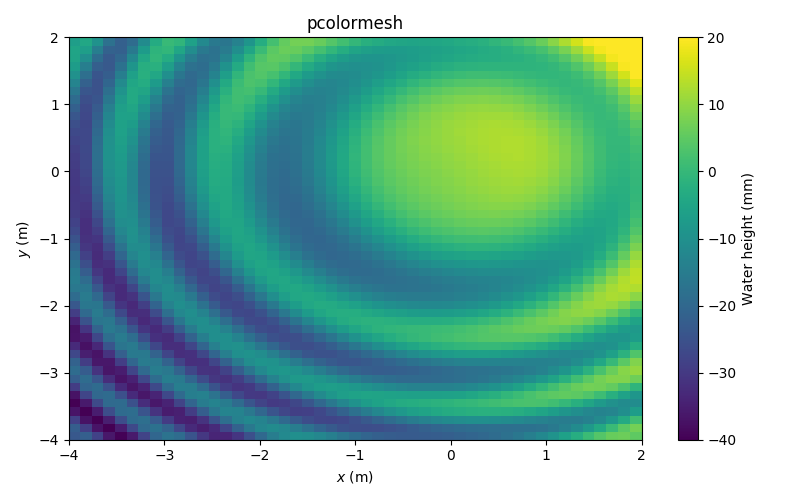
\includegraphics[width=.95\textwidth]{plots/2D_types/pcolormesh.png}
\begin{lstlisting}[language=Python]
plt.pcolormesh(x, y, data, vmin=-40, vmax=20)
plt.colorbar(label='Water height (mm)')
\end{lstlisting}
\end{frame}


\begin{frame}[fragile]
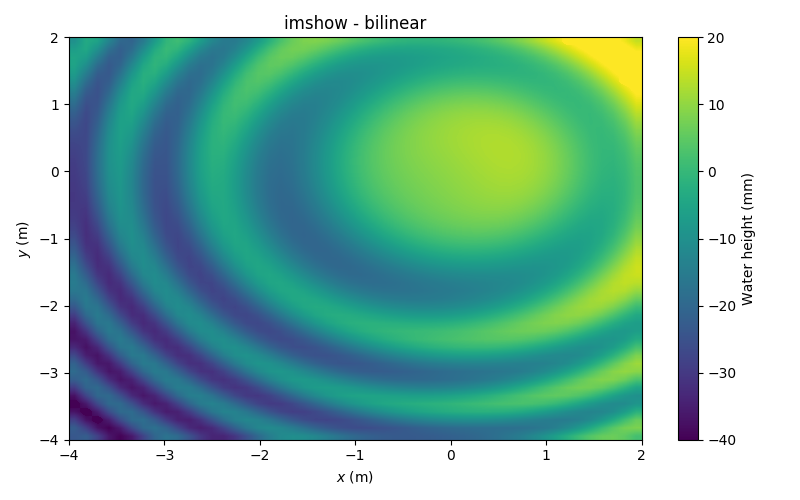
\includegraphics[width=.95\textwidth]{plots/2D_types/ims_bilinear.png}
\begin{lstlisting}[language=Python]
plt.imshow(data, interpolation='bilinear', origin='lower',
  aspect='auto', extent=[x.min(), x.max(), y.min(), y.max()],
  vmin=-40, vmax=20)
plt.colorbar(label='Water height (mm)')
\end{lstlisting}
\end{frame}

\begin{frame}[fragile]
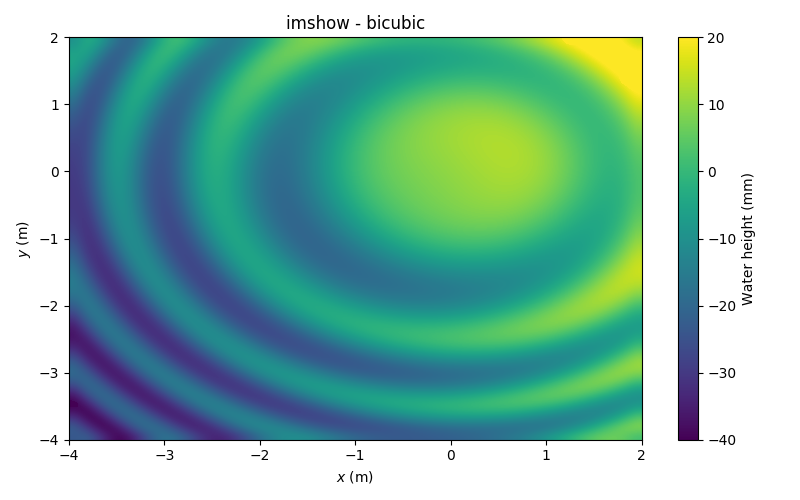
\includegraphics[width=.95\textwidth]{plots/2D_types/ims_bicubic.png}
\begin{lstlisting}[language=Python]
plt.imshow(data, interpolation='bicubic', origin='lower',
  aspect='auto', extent=[x.min(), x.max(), y.min(), y.max()],
  vmin=-40, vmax=20)
plt.colorbar(label='Water height (mm)')
\end{lstlisting}
\end{frame}



\slide{Sometimes the interpolation can make a big difference}{
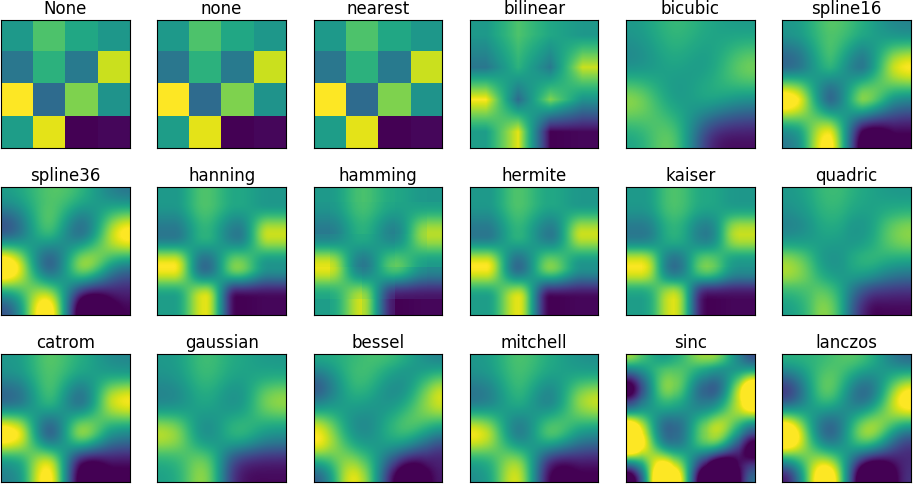
\includegraphics[width=\textwidth]{plots/2D_types/interpolation_ex_plt2.png}

Taken from \citet{plt_gallery}.
}

\begin{frame}[fragile]
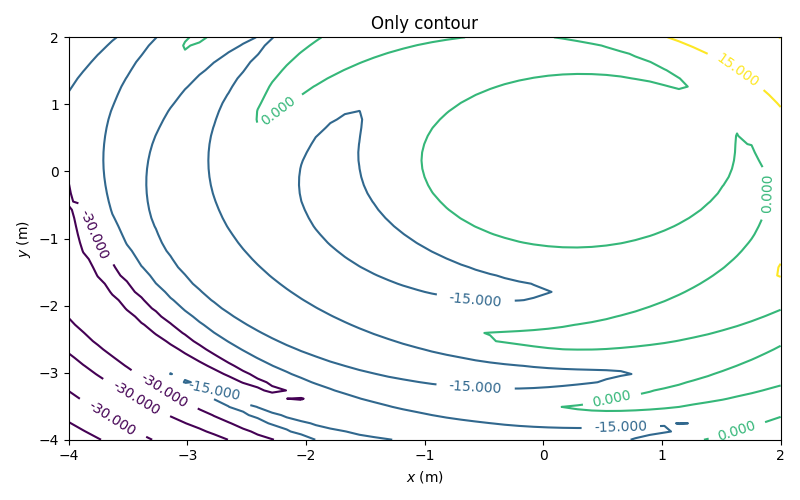
\includegraphics[width=.95\textwidth]{plots/2D_types/contour.png}
\begin{lstlisting}[language=python]
CS = plt.contour(x, y, z, 5)
plt.clabel(CS, inline=1, fontsize=10)
\end{lstlisting}
\end{frame}


\begin{frame}[fragile]
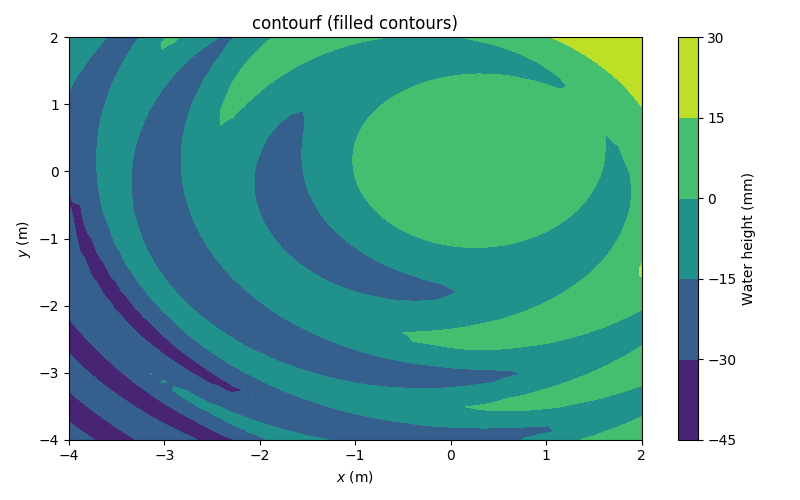
\includegraphics[width=.95\textwidth]{plots/2D_types/contourf.png}
\begin{lstlisting}[language=python]
plt.contourf(x, y, z, 5)
plt.colorbar(label='Water height (mm)')
\end{lstlisting}
\end{frame}

\begin{frame}[fragile]
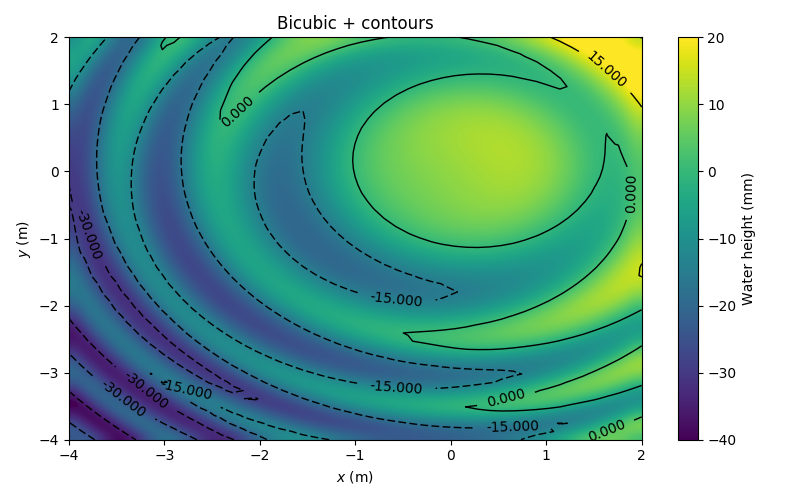
\includegraphics[width=.95\textwidth]{plots/2D_types/ims_bicubic_contour.png}
\begin{lstlisting}[language=python]
plt.imshow(z, interpolation='bicubic', origin='lower', 
    extent=[-4,2,-4,2], aspect='auto', vmin=-40, vmax=20)
plt.colorbar(label='water height (mm)')
cs = plt.contour(x, y, z, 5, colors='black', linewidths=1.0)
plt.clabel(cs, inline=1, fontsize=10)
\end{lstlisting}
\end{frame}



\subsection{Types of plot (flow)}

\begin{frame}[fragile]
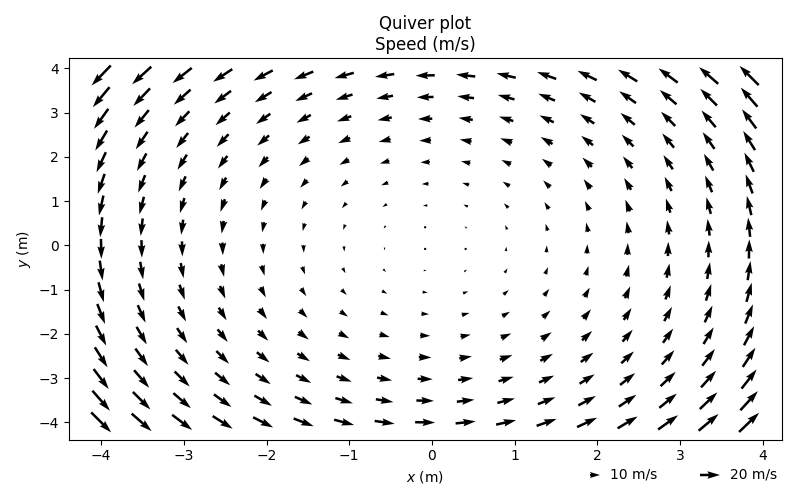
\includegraphics[width=.95\textwidth]{plots/2D_types/quiver.png}
\begin{lstlisting}[language=python]
Q = plt.quiver(x, y, U, V, pivot='mid',
    scale_units='dots', scale=1)
plt.quiverkey(Q, 0.9, 0.05, 20, r'20 m/s',
    labelpos='E', coordinates='figure')
plt.quiverkey(Q, 0.75, 0.05, 10, r'10 m/s',
    labelpos='E', coordinates='figure')
\end{lstlisting}
\end{frame}

\begin{frame}[fragile]
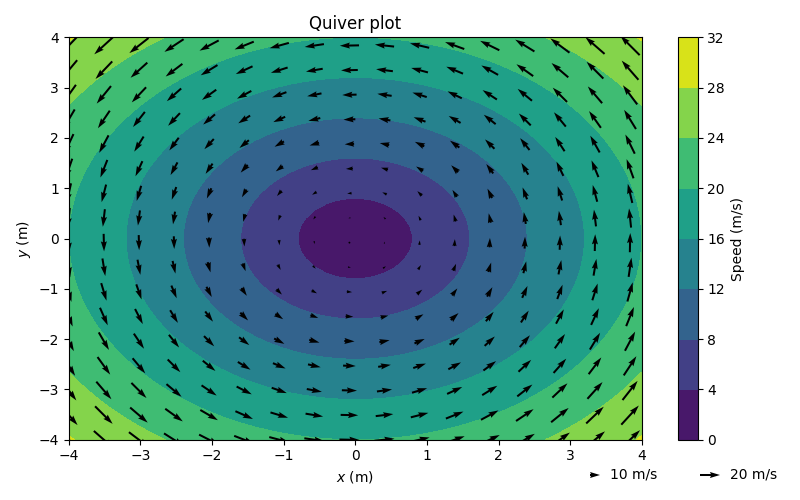
\includegraphics[width=.95\textwidth]{plots/2D_types/quiver_contourf.png}
\begin{lstlisting}[language=python]
plt.contourf(x,y,speed)
plt.colorbar(label='Speed (m/s)')
Q = plt.quiver(x, y, U, V, pivot='mid',
    scale_units='dots', scale=1)
plt.quiverkey(Q, 0.9, 0.05, 20, r'20 m/s',
    labelpos='E', coordinates='figure')
plt.quiverkey(Q, 0.75, 0.05, 10, r'10 m/s',
    labelpos='E', coordinates='figure')
\end{lstlisting}
\end{frame}



\begin{frame}[fragile]
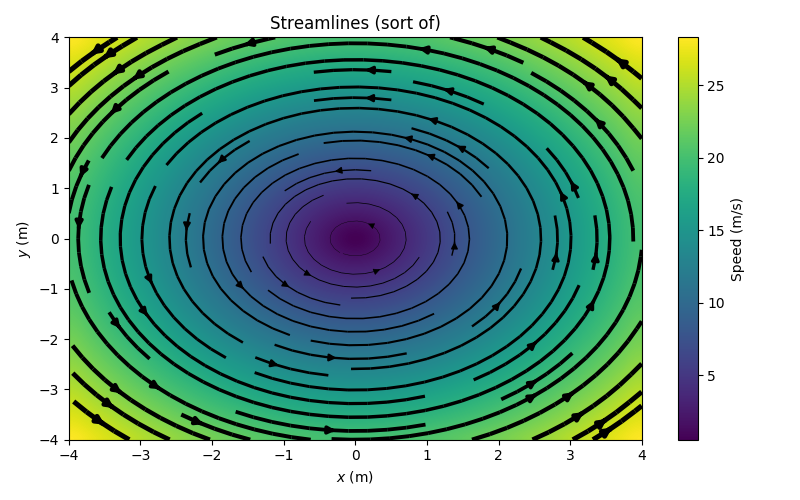
\includegraphics[width=.95\textwidth]{plots/2D_types/streamlines.png}
\begin{lstlisting}[language=python]
plt.imshow(speed, origin='power', interpolation='bicubic',
    extent=[x.min(),x.max(),y.min(),y.max()], aspect='auto')
plt.colorbar(label='Speed (m/s)')
plt.streamplot(x,y,U,V, linewidth=nspeed, color='k')
\end{lstlisting}
\end{frame}


\begin{frame}[fragile]
\centering
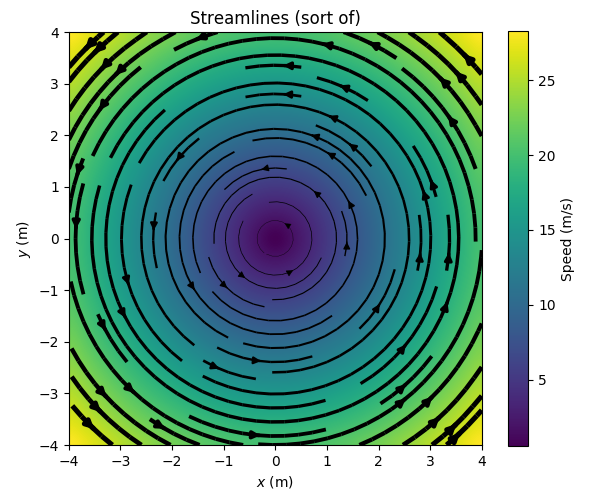
\includegraphics[width=.85\textwidth]{plots/2D_types/streamlines_equal.png}
\begin{lstlisting}[language=python]
plt.imshow(speed, origin='power', interpolation='bicubic',
    extent=[x.min(),x.max(),y.min(),y.max()], aspect=1)
plt.colorbar(label='Speed (m/s)')
plt.streamplot(x,y,U,V, linewidth=nspeed, color='k')
\end{lstlisting}
\end{frame}






\subsection{Colormaps}


\slide{The color scale is important}{

\begin{itemize}
\item Prefer a scale that has continuous color perception
\item Scale depends on the characteristic of your data (clear +/- dichotomy?)
\item Plotting log also might be useful
\end{itemize}


\movie[label=cells,width=4cm,poster,showcontrols,externalviewer=vlc]{Different
colormaps animation}{movies/goldbaum-galaxies-all-colormaps.mkv}
}


\begin{frame}[fragile]{Jet colormap}
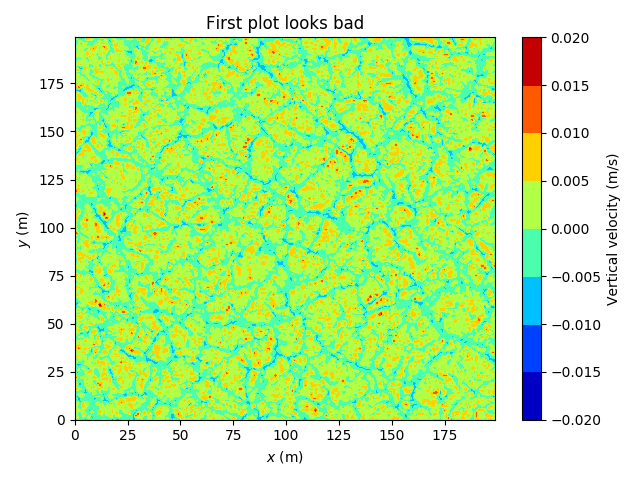
\includegraphics[width=.95\textwidth]{plots/cmaps/jet.png}
\begin{lstlisting}
plt.contourf(w0, cmap='jet') 
\end{lstlisting}
\end{frame}


\begin{frame}[fragile]{Viridis colormap}
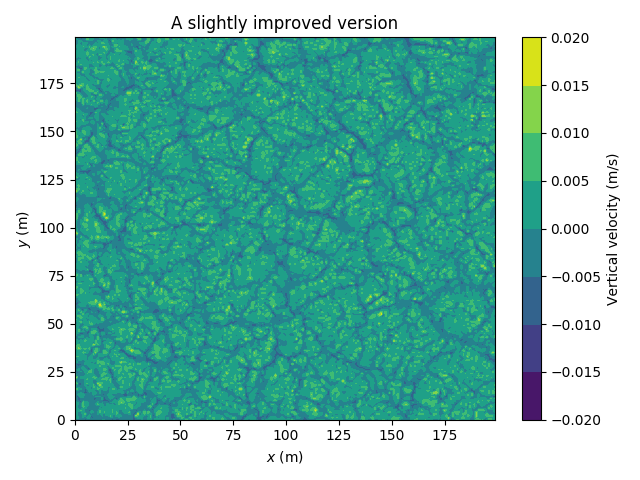
\includegraphics[width=.95\textwidth]{plots/cmaps/viridis.png}
\begin{lstlisting}
plt.contourf(w0, cmap='viridis') 
\end{lstlisting}
\end{frame}


\begin{frame}[fragile]{Symmetric (divergent) colormap}
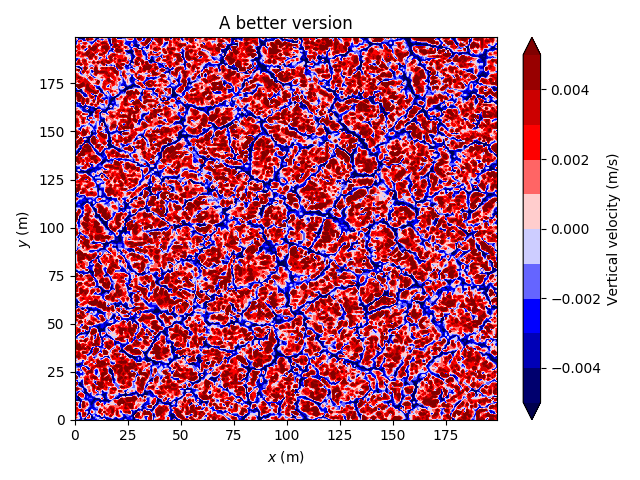
\includegraphics[width=.95\textwidth]{plots/cmaps/rdbu.png}
\begin{lstlisting}
plt.contourf(w0, cmap='seismic') 
\end{lstlisting}
\end{frame}



\slide{Some features might be easier to see}{
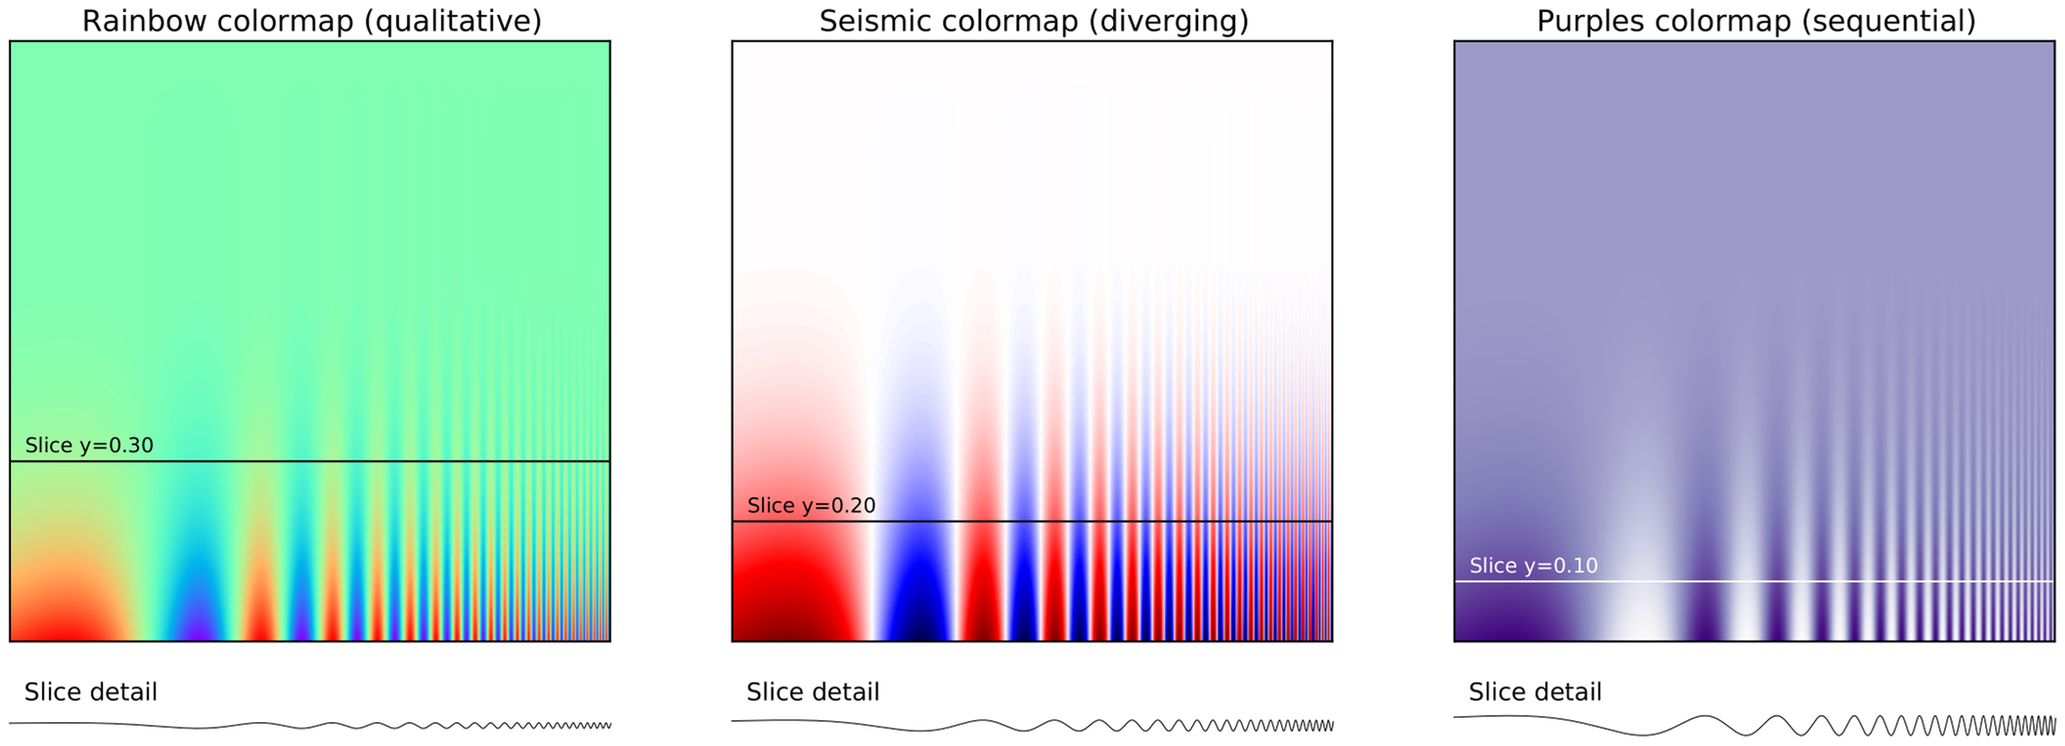
\includegraphics[width=\textwidth]{plots/colormap_blue2.png}

Taken from \citet{rougier.ea2014}.
}


\section{3D data (animations)}

\begin{frame}[fragile]
\movie[label=cells,width=4cm,poster,showcontrols,externalviewer=vlc]{Temperature
animation}{movies/T_surf.mp4}
\begin{lstlisting}[language=python]
# Data reading happens before this
fig = plt.figure()
ims = []

for it in range(300):
    im = plt.imshow(T[it], animated=True, cmap='viridis',
      origin='lower', extent=[0, 1e3, 0, 1e3],
      vmin=T.min(), vmax=T.max(), interpolation='bicubic')
    tx = im.axes.text(0, 0, 'Timestep: {}'.format(it),
      color='black')
    ims.append([im, tx])

plt.colorbar(label='T (K)')
plt.xlabel('$x$ (m)')
plt.ylabel('$y$ (m)')
plt.title('Temperature at the top of a convective ocean')
plt.tight_layout()
ani = animation.ArtistAnimation(fig, ims, interval=50,
  blit=True, repeat_delay=1000)
ani.save('T_surf.mp4', dpi=150)
\end{lstlisting}
\end{frame}


\begin{frame}[fragile]
\movie[label=cells,width=4cm,poster,showcontrols,externalviewer=vlc]{Oil
animation}{movies/C_linear.mp4}
\begin{lstlisting}
# Data reading happens before this
fig = plt.figure()
ims = []
for it in range(300):
    im = plt.imshow(C[it], animated=True, cmap='plasma',
      origin='lower', extent=[0, 1e3, 0, 1e3],
      vmin=0., vmax=10., interpolation='bicubic')
    tx = im.axes.text(0, 0, 'Timestep: {}'.format(it),
      color='white')
    ims.append([im, tx])

plt.colorbar(label='Oil Concentration (kg/m$^3$)')
plt.xlabel('$x$ (m)')
plt.ylabel('$y$ (m)')
plt.title('Concentration at the top of a convective ocean')
plt.tight_layout()
ani = animation.ArtistAnimation(fig, ims, interval=50,
  blit=True, repeat_delay=1000)
ani.save('C_linear.mp4', dpi=150)
\end{lstlisting}
\end{frame}

\begin{frame}[fragile]
\movie[label=cells,width=4cm,poster,showcontrols,externalviewer=vlc]{Oil
animation}{movies/C_log.mp4}
\begin{lstlisting}
# Data reading happens before this
from matplotlib.colors import LogNorm
fig = plt.figure()
ims = []
for it in range(300):
    im = plt.imshow(C[it], animated=True, cmap='plasma',
      origin='lower', extent=[0, 1e3, 0, 1e3],
      vmin=1.e-4, vmax=10., interpolation='bicubic',
      norm=LogNorm())
    tx = im.axes.text(0, 0, 'Timestep: {}'.format(it),
      color='white')
    ims.append([im, tx])

plt.colorbar(label='Oil Concentration (kg/m$^3$)')
plt.xlabel('$x$ (m)')
plt.ylabel('$y$ (m)')
plt.title('Concentration at the top of a convective ocean')
plt.tight_layout()
ani = animation.ArtistAnimation(fig, ims, interval=50,
  blit=True, repeat_delay=1000)
ani.save('C_log.mp4', dpi=150)
\end{lstlisting}
\end{frame}

\slide{Final comments}{
\begin{itemize}
\item Slides and scripts are going to be available
\item Written in Python3, but should work with Python2
\end{itemize}
}

\section*{}
\slide{}{\printbibliography}

\end{document}
